% Chapter 1

\chapter{Introduction} % Main chapter title
\label{Chapter1} % For referencing the chapter elsewhere, use \ref{Chapter1} 

This chapter presents a panoramic view of the field of study on which this thesis
bases itself.
First we introduce the fundamental concepts of machine learning, followed by
some more topic-specific discussion, then an overview of the main contribution
is given, followed by the document outline.

\section{Relationship between data and knowledge}

The current amount of digital data produced daily is estimated to be in the realm of 
ZettaBytes ($1~ZB = 10^{12}~GB$) \cite{idc}.
Of this amount, only a small fraction sees actual processing and interpretation,
mainly because while the flow of information is steady, the available resources
devoted to the task are often limited \cite{idc}.
Moreover in some cases the rapidity at which a meaningful interpretation of the 
raw data has to be produced is critical.
Hence, just the plain fact of owning the data does not implies that some useful 
meaning can be derived from it; in fact a whole discipline was born with the
intent of derive \emph{knowledge} that ``we don't know we don't know''.

This is indeed one of the many achievement of \emph{Data Mining}, a prominent field for
professionals and scientists alike.
Most of its techniques draw from a variety of other fields like Statistics,
Computer Science, Information Theory and Mathematics just to mention a few.
This discipline rests its theoretical foundation upon the field of \emph{Machine Learning},
the discipline that studies algorithms and techniques that allows a machine
to learn a concept (or an approximation of it) from a set of examples.
These algorithms start from limited evidence and try to build up a general model
by refining an initial hypothesis.
Machine Learning is mostly useful when either an exact solution to a very
difficult problem is computationally infeasible or the problem specification
is rather vague or not unambiguously defined, leaving to the algorithm the burden
of exploration.

One of the pivotal concepts of this field is data \emph{representation}.
For the most part, data is collected and stored in vectorial form (think of
a database rows for instance) and a lot of machine learning techniques are
tailored to this ubiquitous representation.
A vector is just a tuple of values with some kind of identifier for each of them
and represent little to no other information per se hence data that comes in
this format is considered unstructured data.

In the last decades some approaches tried to address tasks whose data could
not be represented in vectorial form or whose representation this way would cause
a great deal of information loss.
More specifically some work has been done to devise methods that could learn
directly from graphs, a very useful kind of \emph{structured data} that sees many
important real-world applications nowadays, especially in Biology and Chemistry.

%----------------------------------------------------------------------------------------

\section{Why structured data}
As previously mentioned, data in vectorial form retain practically no inherent
information about the record it represent, it's just a collection of values with
no other relation between themselves but to be in the same tuple.
Looking at a vector for instance, it is not immediately clear if the values share
some dependency, if they are correlated and in which measure, and what is the
individual relevancy to the prediction task at hand, if any.
To overcome these question a number of analyses exist, which aim to add some
implicit knowledge to the data but they remain heuristic at best.

\subsection{Graph representation}
On the other hand we have graphs, a structured data form that can represent
a great deal of different information depending on the domain of application.
Graphs have different level of information semantics and each level has not an
unique connotation either, e.g. consider the set of edges, they could represent
different notions of relationship between the nodes while maintaining the same
representation.
Beside the above mentioned edges, which express a kind of local ``relationship''
information between the nodes, we have information stored at the node level, in the
labels were some actual qualitative or quantitative data akin to the vectorial
counterpart may be present.
Graph-wise, at a more global level we have topological information, which can be
viewed like an extended relationship level, and finally the information that can
be derived or inferred by looking at the shape of the graph such that notions
of connectivity, density etc.

Since this thesis will focus on data encoded as graphs we will now introduce
some examples of learning tasks on graphs.  

\subsubsection{Examples}

Graph structured data has proven useful in the classification of non-coding RNA
molecules, modeled as shown in Figure \ref{fig:bio} \cite{nnavarin, conf/psb/KarklinMH05},
also, the present study experimental part is conducted on datasets that represent
molecules of some sort in form of graphs.

\begin{figure}[ht]
    \centering
    \begin{subfigure}{.4\textwidth}
        \centering
        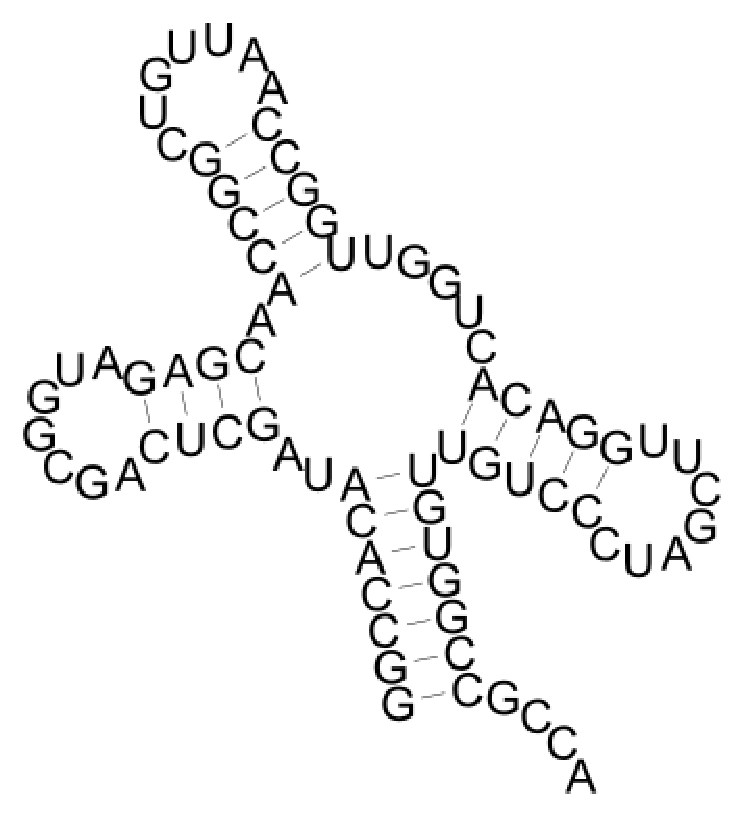
\includegraphics[width=\linewidth]{Figures/rna}
        \label{fig:rna}
        \caption{}
    \end{subfigure}
    \begin{subfigure}{.4\textwidth}
        \centering
        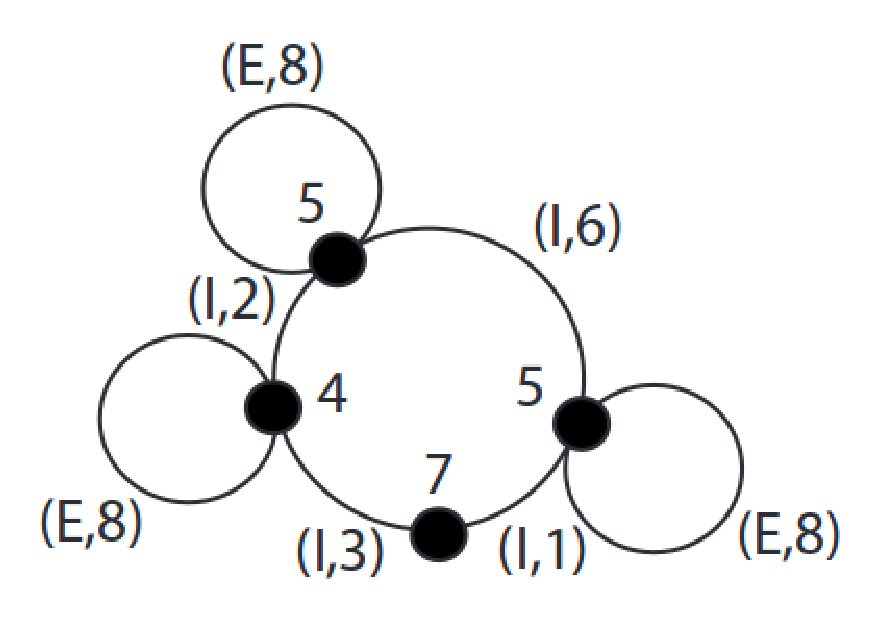
\includegraphics[width=\linewidth]{Figures/ldgrna}
        \label{fig:ldg}
        \caption{}
    \end{subfigure}
    \caption{A) RNA molecule graph representation and B) the same molecule represented
        as a labeled dual graph \cite{conf/psb/KarklinMH05}.}
    \label{fig:bio}
\end{figure}

Natural language processing is another field were graph representation is often used
as the basis for elaborate meaning extraction, as is the case for building opinion
lexicon from users review \cite{10.1371/journal.pone.0079294}, see Figure \ref{fig:wordrel}.

\begin{figure}[ht]
    \centering
    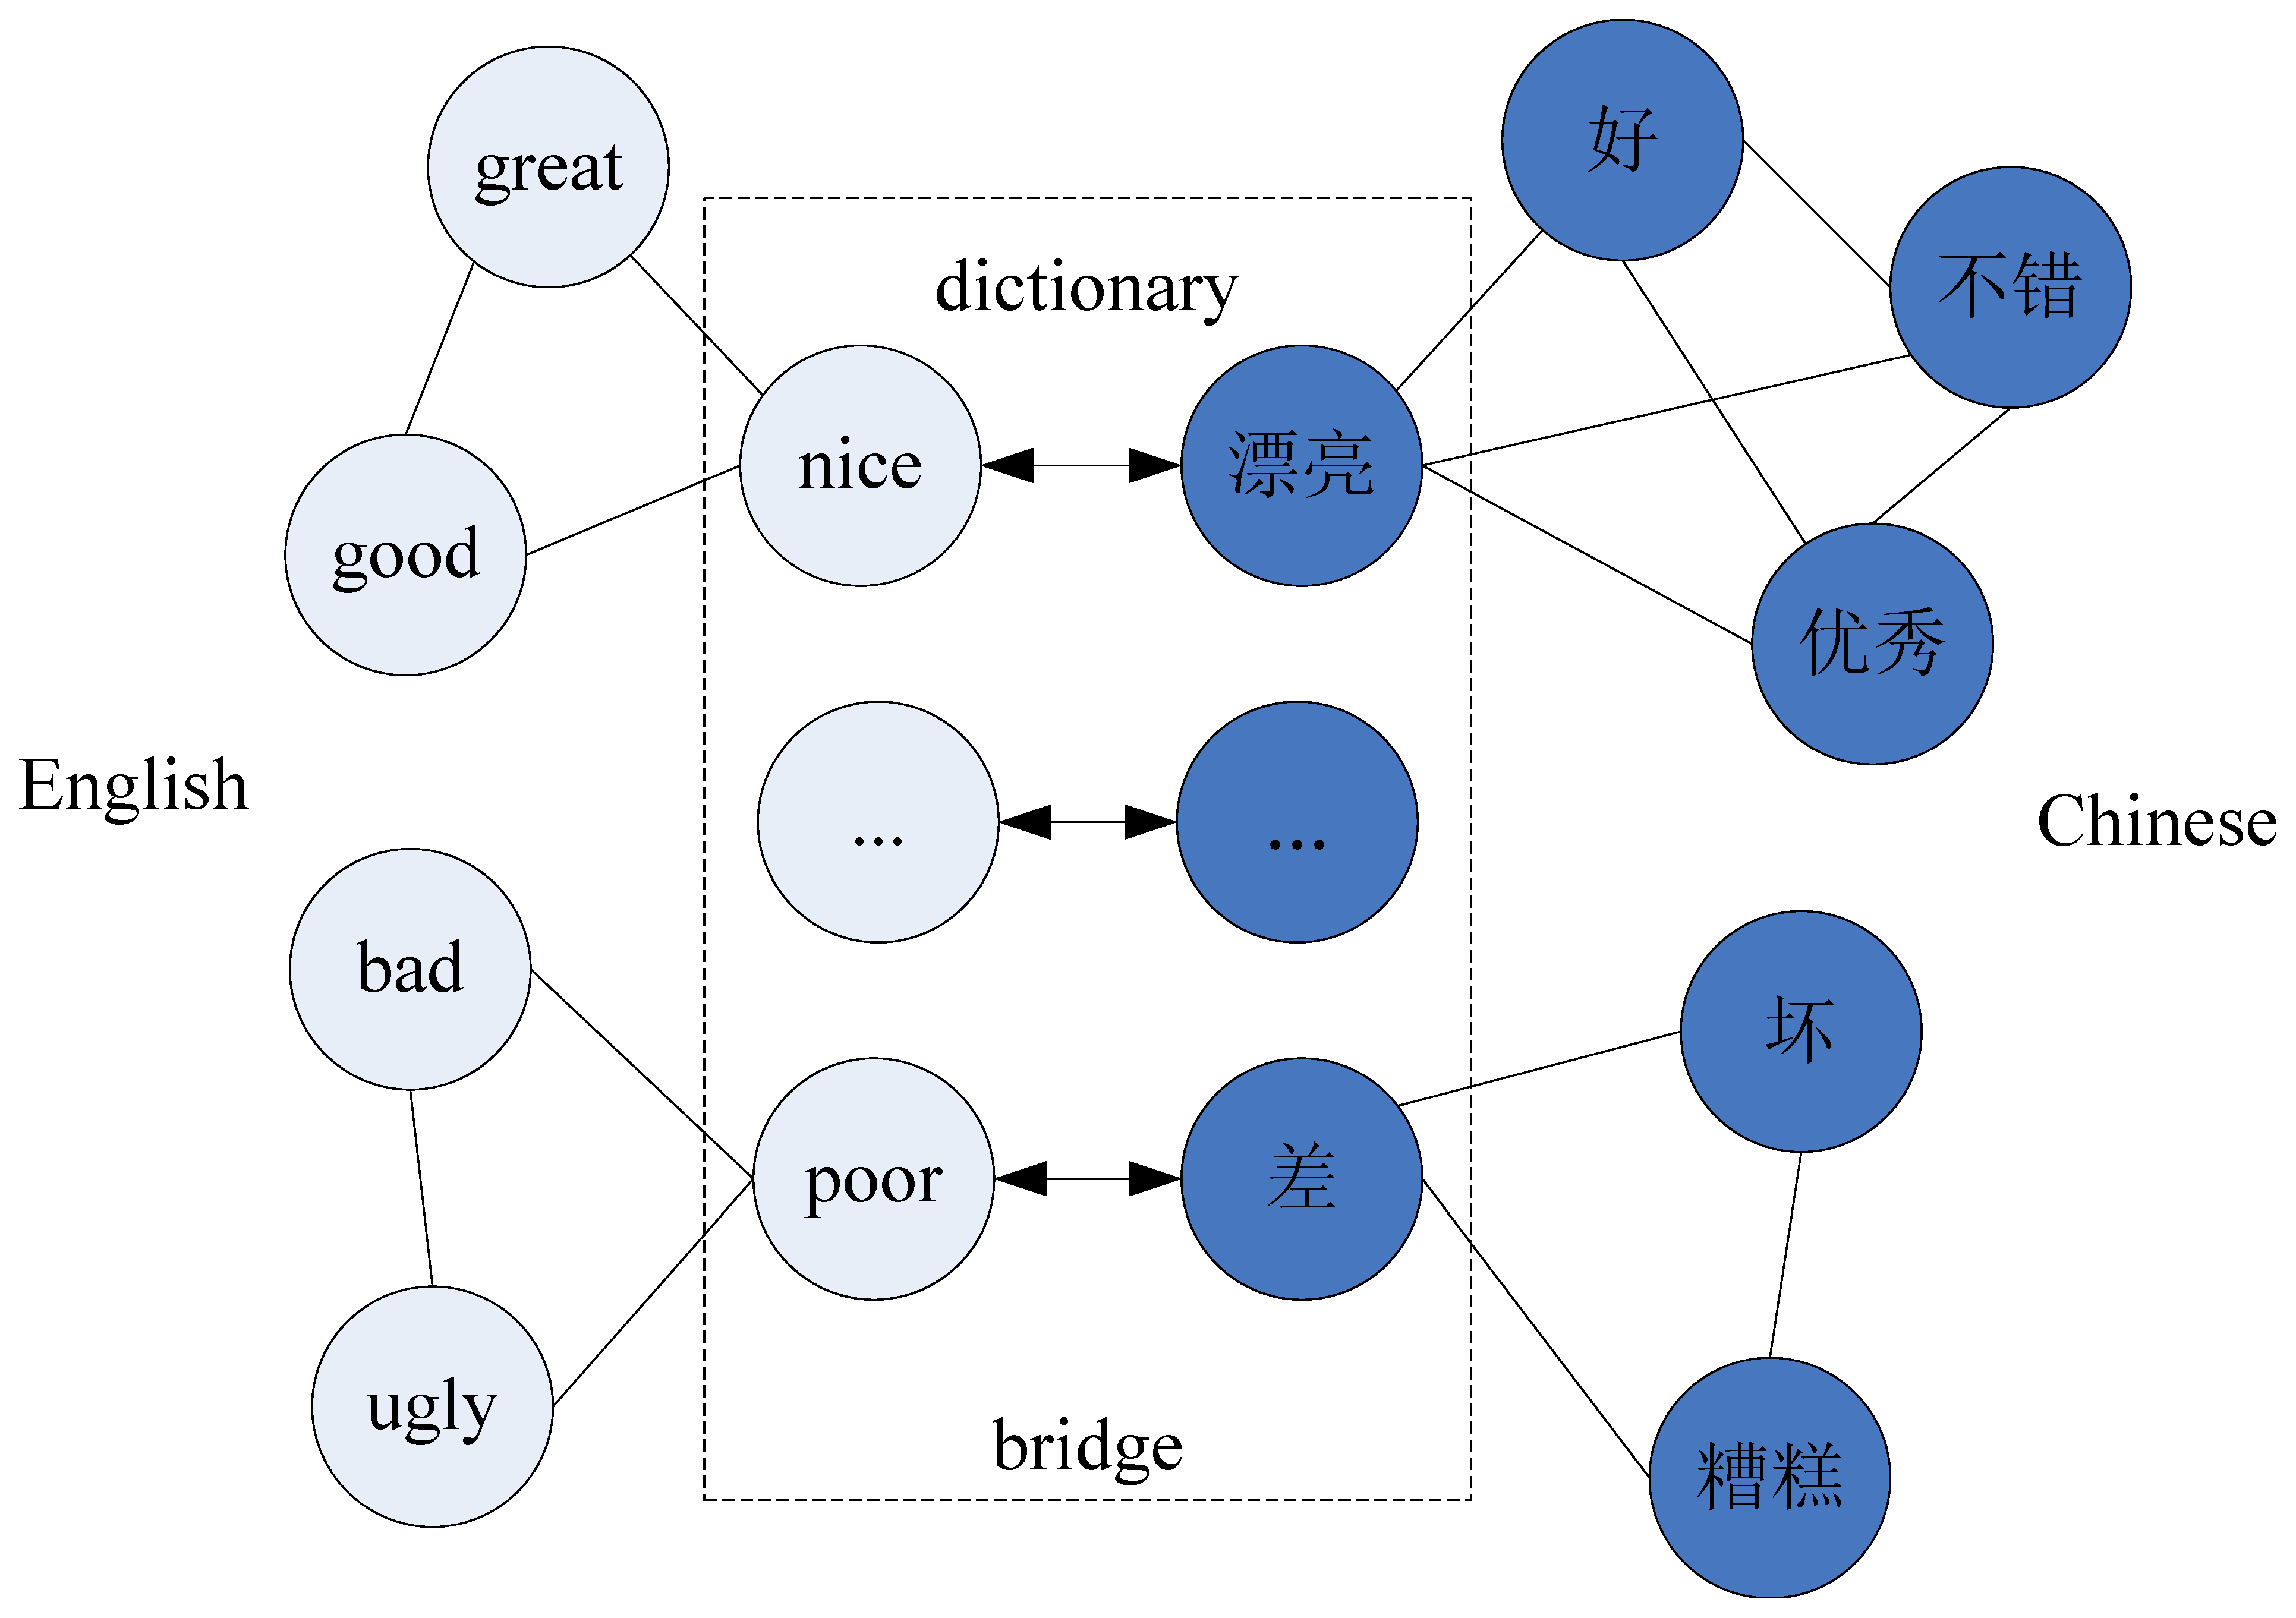
\includegraphics[width=.6\linewidth]{Figures/wordrel}
    \label{fig:wordrel}
    \caption{Example of mutual-reinforcement label propagation using a graph
    representation of words relationships in a multilingual context \cite{10.1371/journal.pone.0079294}.}
\end{figure}

In computer vision a prominent application of the graph representation concerns
the so called scene understanding or scene modelling task, where a scene is divided
into semantically meaningful areas which can be seen as nodes of a graph whose
edges are the adjacency relations between the areas \cite{journals/corr/abs-1108-4079},
an exemplification of which is given in Figure \ref{fig:scene}.

\begin{figure}[ht]
    \begin{subfigure}{.45\linewidth}
        \centering
        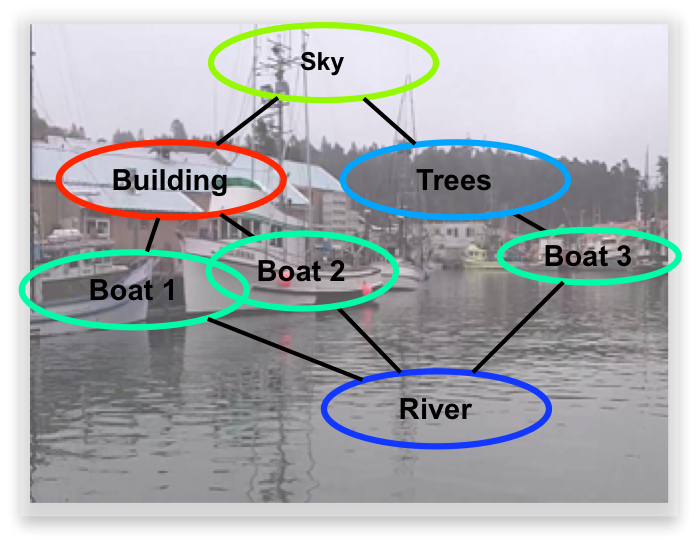
\includegraphics[width=\linewidth]{Figures/scene}
        \caption{}
        \label{fig:scene}
    \end{subfigure}
    \begin{subfigure}{.45\linewidth}
        \centering
        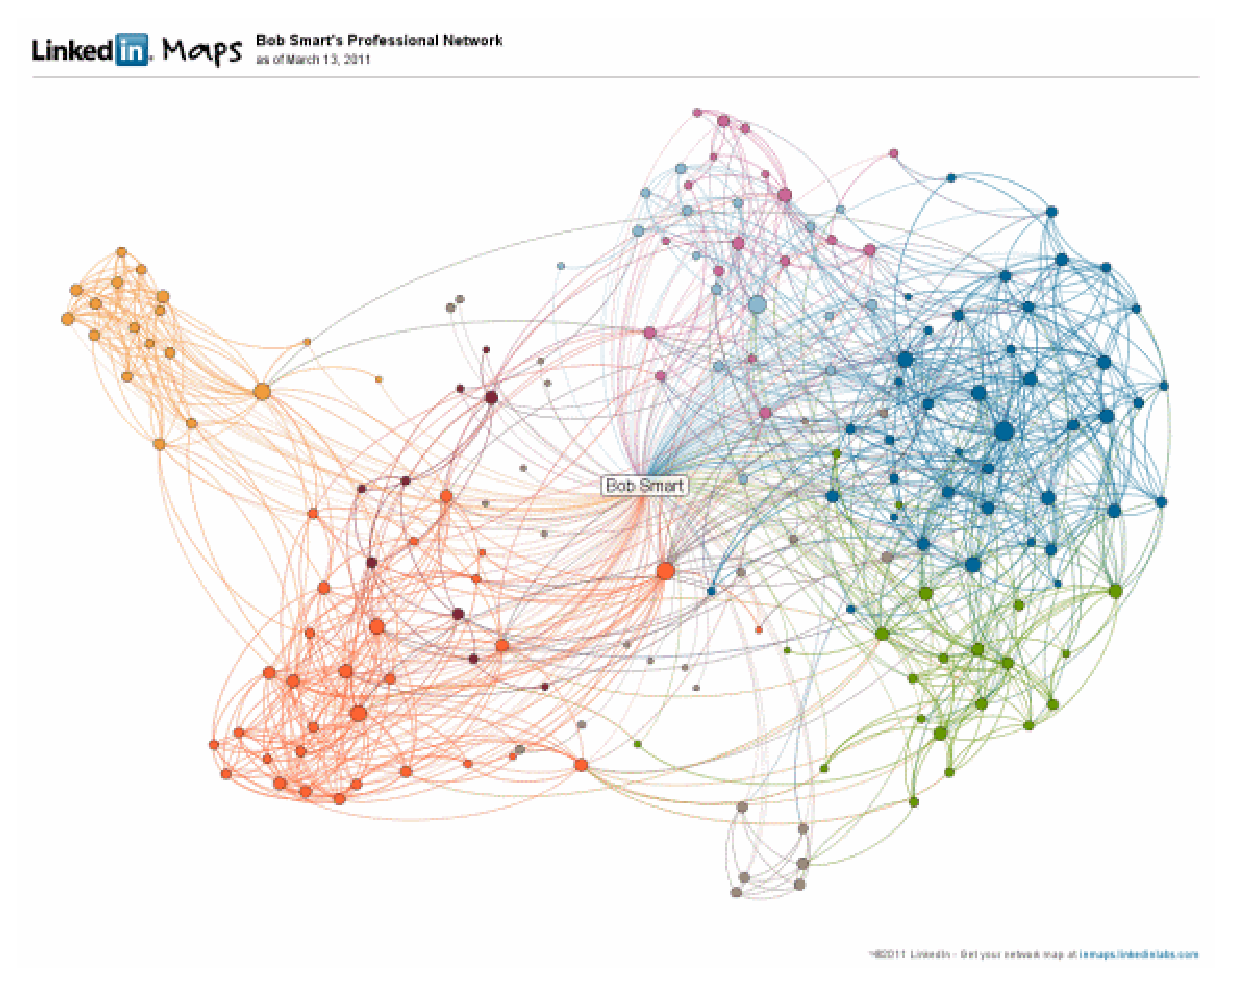
\includegraphics[width=\linewidth]{Figures/linkedin-social-maps}
        \caption{}
        \label{fig:network}
    \end{subfigure}
\caption{A) Scene understanding via graph decomposition in computer vision. B)
        LinkedIn's social maps show how a social network graph representation
        can quickly become very complex.}
\end{figure}

Finally  the graphs deriving from the inherently structured organization of every social
network can lead to a large number of mining possibilities given also the vast
amount of data available \cite{gundecha2012mining}.
Figure \ref{fig:network} gives an example of social network derived from a real-world
application.

%----------------------------------------------------------------------------------------

\section{Kernel methods}
Graph mining and in general machine learning approaches that deal with data
structured as graphs are still an active area of research for a number of reason
detailed in Chapter \ref{Chapter2}, here we will just mention the trade-off
associated with devising methods that are effective while remaining feasible.
Some of the recently proposed works \cite{DBLP:conf/sdm/MartinoNS12, NIPS2009_3813}
try to embed graph specific knowledge and theories into well established methods,
in particular kernel methods that, given the inherent decoupling between the kernel
function and the learning machine that employs it, have seen a wealth of proposal
to address several applications among which there are some of those described in
the previous section.

Nowadays a scientist that wants to address a particular classification task
typically has to first determine which is the best approach to choose given a number
of factors including data representation, amount of samples, and type of prediction.
Again, the outcome of the experiments conducted with the method of choice has 
to go a rigorous path of validation and testing to ensure significance not to
mention correctness.
In particular this last point can quickly become a cumbersome and onerous process if
it is unclear which one of the available alternative methods is the most indicated
for the task at hand, and this becomes even more true if the choice concerns a 
kernel function.

To address this latter point in the recent years some algorithms have been developed
\cite{journals/jmlr/GonenA11} that consent to combine different kernel functions into a single learning
process, trying in some way to ease the burden of choice that affects the user.
In the following section we will describe our proposal, which tries to improve on
the existing technique by extending the notion of kernel combination in a way which
to the author's knowledge has yet to be done.

%----------------------------------------------------------------------------------------

\section{Thesis contribution}

The scenario described in the previous section prompted us to try and devise a way to
overcome some of the weak points in the general kernel learning methodology, namely
the overall efficiency, in particular when graph kernel learning is involved.
We tried furthermore to prove the generalizability of this methodology via empirical
testing, see Chapter \ref{Chapter4}.

\subsection{Why combining kernels}
\label{sec:why}
% relieve the burden of kernel design from the user that can mash a number of weak kernels
% in and expect something out
% vedi paper easymkl

Kernel combination can stem from multiple needs, here we will briefly mention the main ones.

\paragraph{Relieve the user from deep domain specific knowledge:} in order to be able to design
adequate kernels for the problem at hand a user needs to to delve into the details of the data
and the concept it is trying to approximate, making the choice of a kernel a hindering task.
Combining multiple, possibly weaker, kernels will in principle overcome this difficulty with
a null or modest loss in performances.
\paragraph{Combine heterogeneous sources of information:} one kernel means one mapping function
toward a particular high dimensional space, thus inducing a whole new feature set.
Different data sources for the same task could have different notions of similarity,
thus requiring the employment of a different kernel.
Having the possibility to combine different kernels in one learning process equals
to combine different feature sets from (possibly) different sources.
\paragraph{Features selection:} depending on the chosen method of combination, it could be
possible in principle to still measure the performance of the single kernel according
to some metrics hence being able to assess the goodness of the underling input feature space.
\paragraph{The case for graph kernels:} graph kernels typically suffer a performance
degradation the more expressive they get. By combining a number of more efficient although
less expressive kernels could lead to a boost in performance due to the inherent enrichment
of the feature set while maintaining acceptable performances.

\subsection{Proposed solution}

The solution proposed here consists in combining the kernels that would be
generated according to a grid search technique (see Section \ref{subsubsec:grid})
all at once, thus extending the notion of combination to kernels generated by the same
function but from different parameters, while employing a specific technique to
improve the feature space of each kernel and reduce the overall number of computed
matrices.
We had available a fast, state-of-art $MKL$ implementation \cite{aiolli2015easymkl}
so we decided to exploit the inherent combining power of this approach for our
purposes.

By combining a large number of kernels, derived from selected graph kernel
learning approaches, into a single learning process we wanted to determine if an
effective and overall performance improvement both in computational times and 
in target prediction was possible.

Moreover in this way the whole process of parameters selection has been streamlined and
lifted from the kernels to the learning machine, effectively eliminating the need to test each
kernel in isolation.

%----------------------------------------------------------------------------------------

\section{Thesis outline}
This document is organized in five chapters which are: the present one of introduction,
where we explained some of the motives behind this work and the proposed ideas.
In Chapter \ref{Chapter2} we will delve into the background details that will be
necessary to fully understand the later concepts; we will cover the basics of
machine learning and kernel methods and see some examples of kernel combination
techniques.
The main ideas behind this work are exposed in Chapter \ref{Chapter3} where we
discuss in detail our approach, the conceptual steps involved and the solutions
to the problems encountered.
Chapter \ref{Chapter4} covers the experimental part of the thesis, where we present
our results and finally Chapter \ref{Chapter5} wraps it up and contains some of the
ideas that we were not able to include in the present work because of time constraints.


%----------------------------------------------------------------------------------------

% vim: spell spelllang=en_gb
